\documentclass[sigconf,nonacm]{acmart}

\setcopyright{none}
\settopmatter{printacmref=false}
\renewcommand\footnotetextcopyrightpermission[1]{}
\pagestyle{plain}

\usepackage{booktabs}
\usepackage{tabularx}
\usepackage{tikz}
\usetikzlibrary{shapes.geometric,arrows.meta,positioning,fit,backgrounds,calc}
\usepackage{url}
\urlstyle{rm}

\definecolor{cblue}  {RGB}{ 70,120,200}
\definecolor{cgreen} {RGB}{ 50,160, 80}
\definecolor{corange}{RGB}{210,120, 30}
\definecolor{cred}   {RGB}{200, 60, 50}
\definecolor{cgray}  {RGB}{100,100,100}

\begin{CCSXML}
<ccs2012>
  <concept><concept_id>10002978.10003014</concept_id>
    <concept_desc>Security and privacy~Software security engineering</concept_desc>
    <concept_significance>500</concept_significance></concept>
  <concept><concept_id>10011007.10011074.10011099</concept_id>
    <concept_desc>Software and its engineering~Software verification and validation</concept_desc>
    <concept_significance>500</concept_significance></concept>
  <concept><concept_id>10011007.10011074.10011134</concept_id>
    <concept_desc>Software and its engineering~Software maintenance</concept_desc>
    <concept_significance>300</concept_significance></concept>
</ccs2012>
\end{CCSXML}
\ccsdesc[500]{Security and privacy~Software security engineering}
\ccsdesc[500]{Software and its engineering~Software verification and validation}
\ccsdesc[300]{Software and its engineering~Software maintenance}

\title{Software Assurance Beyond Secure Coding: Lessons from the 2024 CrowdStrike Global Outage}

\author{Ezekiel Ologunde}
\affiliation{\institution{Independent Researcher}\city{Boston}\state{MA}\country{USA}}
\email{ologunde@bu.edu}

\begin{abstract}
The July 2024 CrowdStrike Falcon Sensor update failure, which crashed millions of Windows
systems globally and disrupted critical infrastructure including aviation, healthcare, and
financial services, exposed fundamental weaknesses in software assurance practices extending
beyond traditional secure coding paradigms. This incident, caused not by malicious actors
but by failed quality assurance processes in the update delivery pipeline, demonstrates that
software security encompasses the entire lifecycle from development through deployment and
operations. Through comprehensive analysis of the CrowdStrike outage, recent NIST SP 800-53
revisions addressing software update controls, and contemporary DevSecOps challenges, this
paper examines how automation amplifies the consequences of quality assurance failures in
modern software systems. We investigate the paradox that defensive security tools can become
disruption vectors when update integrity verification, pre-deployment testing, and rollback
mechanisms are inadequate. Drawing from Software Engineering Institute research on DevSecOps
implementation barriers and NIST's enhanced controls for patch management operational
resilience, we propose a comprehensive framework for software assurance that treats update
pipelines with equivalent scrutiny to initial development. The research demonstrates that
effective software assurance requires shifting from checkpoint-based validation to continuous
lifecycle governance encompassing deployment verification, operational monitoring, and
automated rollback capabilities.
\end{abstract}

\keywords{Software assurance; DevSecOps; patch management; software updates; quality
assurance; operational resilience; CrowdStrike outage; continuous deployment; rollback}

\begin{document}
\maketitle

\section{Introduction}

On July 19, 2024, a routine software update for CrowdStrike's Falcon Sensor endpoint
protection platform triggered one of the most significant IT disruptions in modern history.
The faulty update crashed millions of Windows systems simultaneously, grounding thousands
of flights, halting hospital operations, disrupting financial services, and interrupting
critical business operations worldwide~\cite{plummer2024crowdstrike}. The incident affected
aviation (Delta, United), healthcare (NHS England), financial services, media (Sky News,
ABC), and countless enterprises relying on CrowdStrike for endpoint protection.

What makes this incident particularly instructive is that the disruption resulted not from
a sophisticated cyberattack but from failures in quality assurance processes governing
software update delivery. According to cybersecurity experts, the problematic update likely
skipped necessary quality checks, resulting in logic errors that caused access violations
and memory corruption in production~\cite{siddiqui2024crowdstrike}. A defensive security
tool designed to protect systems became a disruption vector due to inadequate software
assurance in the update pipeline.

This incident illustrates a fundamental paradox: as systems become increasingly automated
and dependent on continuous deployment, the potential consequences of single update errors
amplify exponentially. The CrowdStrike update propagated globally within hours,
demonstrating how modern software distribution architectures can transform localized quality
assurance failures into worldwide operational crises.

\subsection{Research Questions and Contributions}
\sloppy

This paper addresses four fundamental questions: (RQ1)~What software assurance failures
enabled the CrowdStrike update to bypass quality gates? (RQ2)~How do contemporary
DevSecOps practices address assurance requirements for update pipelines? (RQ3)~What
controls are necessary to ensure update delivery maintains standards equivalent to initial
development? (RQ4)~How can organizations balance rapid deployment velocity with
comprehensive quality assurance?

Our contributions include: (1)~comprehensive analysis of the CrowdStrike incident
identifying specific assurance process failures; (2)~examination of the gap between secure
coding and operational software assurance; (3)~synthesis of NIST SP 800-53 revisions and
DevSecOps research into an integrated lifecycle framework; and (4)~a proposal of enhanced
assurance controls specifically designed for automated update delivery.

\section{Background and Related Work}

\subsection{DevSecOps and Security Integration}

DevSecOps integrates security throughout the software development and deployment lifecycle
rather than treating security as a separate final gate~\cite{shahin2021continuous}. Research
by the Software Engineering Institute identifies five primary implementation
challenges~\cite{yankel2022devsecops}: (1)~cultural resistance between development, security,
and operations teams; (2)~tool proliferation and alert fatigue; (3)~lack of security skills
among developers; (4)~speed versus security tensions; and (5)~inadequate metrics and
feedback loops. A significant gap in contemporary DevSecOps is the lack of security
assurance embedded in deployment and update
processes~\cite{rajapakse2022challenges}.

\subsection{Software Update Management}

Software updates fix vulnerabilities, correct bugs, and maintain compatibility, but
updates themselves introduce risks. Research demonstrates that 14--24\% of security patches
contain errors requiring subsequent fixes~\cite{xu2021empirical}. Organizations face a
fundamental tension between deploying updates rapidly to address known vulnerabilities and
thorough testing to prevent update-induced disruptions~\cite{householder2020cvd}.

\subsection{Software Supply Chain Security}

The CrowdStrike incident highlights that supply chain security must encompass not only
protection against malicious tampering but also rigorous quality assurance ensuring
released software functions correctly~\cite{ladisa2023sok,ohm2020backstabbers}. Integrity
verification alone proves insufficient if the intentionally released software contains
critical defects.

\subsection{Chaos Engineering and Resilience}

Chaos engineering deliberately injects failures into production systems to test resilience
and recovery~\cite{basiri2021teaching}. This philosophy applies directly to software update
management: rather than assuming updates will always succeed, resilient systems should
incorporate mechanisms to detect update-induced failures rapidly and automatically roll
back to known-good configurations.

\begin{figure*}[t]
\centering
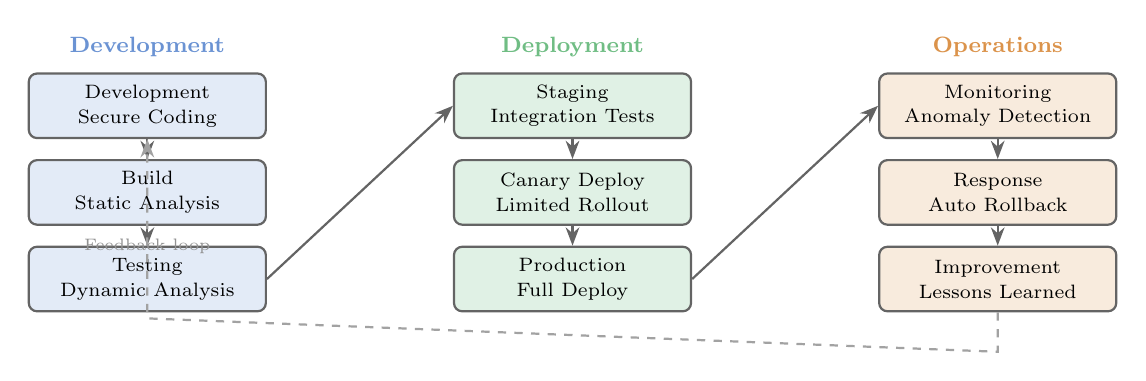
\begin{tikzpicture}[
  font=\fontsize{7pt}{9pt}\selectfont,
  >=Stealth,
  box/.style={rectangle, rounded corners=3pt, draw=cgray, thick,
              minimum width=3.0cm, minimum height=0.82cm,
              text centered, text width=2.8cm, inner sep=3pt},
  arr/.style={-{Stealth}, thick, cgray},
  darr/.style={-{Stealth}, thick, dashed, cgray!60},
  hdr/.style={font=\fontsize{8pt}{10pt}\selectfont\bfseries}
]

  %% ── Column x-centres ─────────────────────────────────────────────────────
  \def\cd{0}    %% Development
  \def\cp{5.4}  %% Deployment
  \def\co{10.8} %% Operations

  %% ── Row y-positions ──────────────────────────────────────────────────────
  \def\yr{0}     %% row 1 (top)
  \def\ym{-1.1}  %% row 2
  \def\yb{-2.2}  %% row 3 (bottom)

  %% ── Phase headers ────────────────────────────────────────────────────────
  \node[hdr, text=cblue!80]   at (\cd, 0.75) {Development};
  \node[hdr, text=cgreen!70]  at (\cp, 0.75) {Deployment};
  \node[hdr, text=corange!80] at (\co, 0.75) {Operations};

  %% ── Development column ───────────────────────────────────────────────────
  \node[box, fill=cblue!15]   (dev)   at (\cd,\yr)  {Development\\Secure Coding};
  \node[box, fill=cblue!15]   (build) at (\cd,\ym)  {Build\\Static Analysis};
  \node[box, fill=cblue!15]   (test)  at (\cd,\yb)  {Testing\\Dynamic Analysis};

  %% ── Deployment column ────────────────────────────────────────────────────
  \node[box, fill=cgreen!15]  (stage)  at (\cp,\yr)  {Staging\\Integration Tests};
  \node[box, fill=cgreen!15]  (canary) at (\cp,\ym)  {Canary Deploy\\Limited Rollout};
  \node[box, fill=cgreen!15]  (prod)   at (\cp,\yb)  {Production\\Full Deploy};

  %% ── Operations column ────────────────────────────────────────────────────
  \node[box, fill=corange!15] (monitor)  at (\co,\yr)  {Monitoring\\Anomaly Detection};
  \node[box, fill=corange!15] (response) at (\co,\ym)  {Response\\Auto Rollback};
  \node[box, fill=corange!15] (improve)  at (\co,\yb)  {Improvement\\Lessons Learned};

  %% ── Down-arrows within columns ───────────────────────────────────────────
  \draw[arr] (dev)    -- (build);   \draw[arr] (build)  -- (test);
  \draw[arr] (stage)  -- (canary);  \draw[arr] (canary) -- (prod);
  \draw[arr] (monitor)-- (response);\draw[arr] (response)--(improve);

  %% ── Cross-column handoff arrows (bottom of each column) ─────────────────
  \draw[arr] (test.east)  -- (stage.west);
  \draw[arr] (prod.east)  -- (monitor.west);

  %% ── Feedback arc: improve → dev (along the bottom, clear of all nodes) ──
  \draw[darr] (improve.south) -- ++(0,-0.5)
    -- (\cd, {(\yb-0.5)})
    -- (dev.south)
    node[midway, below, font=\fontsize{6pt}{7.5pt}\selectfont,
         text=cgray!70]{Feedback loop};

\end{tikzpicture}
\caption{Software assurance lifecycle spanning development, deployment, and operations.
  Effective assurance requires quality gates at each stage with feedback loops enabling
  continuous improvement.}
\label{fig:lifecycle}
\end{figure*}
\subsection{Continuous Integration and Deployment}

Modern software development relies on CI/CD practices that automate building, testing, and
deploying software~\cite{shahin2021continuous}. This automation amplifies the impact of
quality assurance failures, as defects can propagate through automated pipelines to
production before detection~\cite{forsgren2021accelerate}. Common themes across related
incidents (Cloudflare 2019, Facebook 2021, Log4j 2021) include: automation amplifying
failure scope; inadequate pre-production testing; insufficient rollback mechanisms; and
cascading failures from dependent systems.

\section{The CrowdStrike Incident: Analysis}

\subsection{Incident Timeline and Impact}

On July 19, 2024 at approximately 04:09 UTC, CrowdStrike released an update to its Falcon
Sensor via its cloud-based automatic update mechanism~\cite{crowdstrike2024incident}. Within
minutes, Windows systems began experiencing Blue Screen of Death (BSOD) errors and
continuous boot loops: systems would boot, load the faulty Falcon Sensor driver, crash, and
reboot indefinitely~\cite{plummer2024crowdstrike}. Approximately 8.5 million Windows devices
were affected globally~\cite{microsoft2024crowdstrike}, spanning over 5,000 cancelled
flights, NHS and hospital disruptions, financial services outages, and broadcaster
interruptions.

\subsection{Technical Root Cause}

Cybersecurity researchers identified the likely technical cause~\cite{siddiqui2024crowdstrike}:
a logic error in the Falcon Sensor kernel driver caused out-of-bounds memory
access during
driver initialization, triggering Windows kernel exception handling and crashing the system.
The update involved a malformed ``channel file'' (threat detection configuration updated
independently from the core sensor) that the driver could not parse correctly, leading to
null pointer dereferences or invalid memory accesses. Because the Falcon Sensor operates as
a kernel-mode driver with the highest privilege level in Windows, this crash affected the
entire operating system, and because the crash occurred during the boot process, a boot loop
resulted.

\subsection{Software Assurance Process Failures}

Multiple software assurance process failures contributed. Table~\ref{tab:failures}
summarizes the principal failure types and their consequences.

\begin{table}[h]
\caption{Software Assurance Process Failures in the CrowdStrike Incident.}
\label{tab:failures}
\small
\begin{tabularx}{\columnwidth}{@{}p{2.6cm}X@{}}
\toprule
\textbf{Failure Type} & \textbf{Consequence} \\
\midrule
Inadequate Unit Testing  & Memory access violations went undetected \\
\addlinespace[2pt]
Insufficient Static Analysis & Out-of-bounds accesses not flagged \\
\addlinespace[2pt]
Missing Code Review & Logic errors not caught by peers \\
\addlinespace[2pt]
Limited Dynamic Testing & Parsing errors with malformed data not found \\
\addlinespace[2pt]
No Staged Rollout & All systems affected simultaneously \\
\addlinespace[2pt]
Absent Auto-Monitoring & Hours elapsed before global failure detected \\
\addlinespace[2pt]
No Auto-Rollback & Manual remediation required for millions of systems \\
\bottomrule
\end{tabularx}
\end{table}

Comprehensive pre-release testing should have included unit tests detecting memory access
violations, integration tests identifying channel file parsing failures, system tests
revealing the boot-loop failure mode, and regression tests. The simultaneous global
deployment---rather than staged rollout---meant no population-limited canary period to
detect the issue before full exposure. Once the faulty update began causing crashes,
automated mechanisms were absent to correlate the update with the global spike in system
failures and trigger rollback.

\subsection{Sociotechnical Contributing Factors}

Beyond technical failures, security software vendors face pressure to deploy threat
detection updates rapidly, potentially leading to quality shortcuts. The automated update
mechanism that efficiently delivers updates also efficiently delivers faulty ones.
Organizations deploying security software from trusted vendors may also develop complacency
about update risks---the incident demonstrates that even highly reputable vendors can
release defective updates.

\section{DevSecOps Implementation Challenges}

Research identifies lack of security assurance throughout the software development lifecycle
as a primary DevSecOps challenge~\cite{yankel2022devsecops}. Many organizations implement
security activities during development but apply less rigorous validation to deployment
pipelines themselves, creating a paradoxical situation where code is carefully secured but
the delivery mechanism is inadequately secured~\cite{ladisa2023sok}. Figure~\ref{fig:challenges}
enumerates the five key challenges.

\begin{figure}[h]
\centering
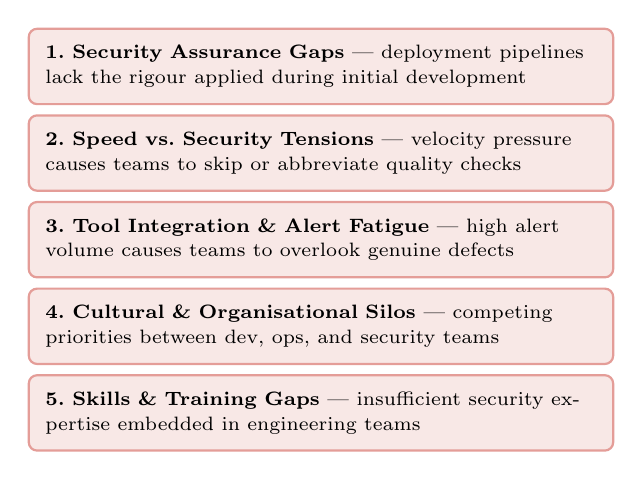
\begin{tikzpicture}[
  font=\fontsize{7pt}{9pt}\selectfont,
  >=Stealth,
  cbar/.style={
    rectangle, rounded corners=3pt, draw=cred!50, thick,
    minimum width=7.2cm, minimum height=0.95cm,
    fill=cred!12, text width=7.0cm,
    align=left, inner sep=6pt
  }
]
  \node[cbar] (c1) at (0, 0.00)
    {\textbf{1.\ Security Assurance Gaps} ---
     deployment pipelines lack the rigour applied during initial development};

  \node[cbar] (c2) at (0,-1.10)
    {\textbf{2.\ Speed vs.\ Security Tensions} ---
     velocity pressure causes teams to skip or abbreviate quality checks};

  \node[cbar] (c3) at (0,-2.20)
    {\textbf{3.\ Tool Integration \& Alert Fatigue} ---
     high alert volume causes teams to overlook genuine defects};

  \node[cbar] (c4) at (0,-3.30)
    {\textbf{4.\ Cultural \& Organisational Silos} ---
     competing priorities between dev, ops, and security teams};

  \node[cbar] (c5) at (0,-4.40)
    {\textbf{5.\ Skills \& Training Gaps} ---
     insufficient security expertise embedded in engineering teams};

\end{tikzpicture}
\caption{Five primary DevSecOps implementation challenges that directly contributed
  to the quality assurance failures enabling the CrowdStrike incident.}
\label{fig:challenges}
\end{figure}

The CrowdStrike incident exemplifies the speed versus security tension: security software
vendors face genuine pressure to deploy threat detection updates rapidly, creating incentive
to abbreviate quality assurance for updates perceived as lower risk. Effective DevSecOps
requires cultural transformation where security becomes a shared responsibility across
development, operations, and security teams~\cite{rajapakse2022challenges}.

\section{NIST SP 800-53 Revisions}

The August 2024 revision to NIST SP 800-53 introduced significant enhancements addressing
software updates~\cite{nist2024sp80053}. Enhanced \textbf{SI-2 (Flaw Remediation)} now
requires update integrity verification via cryptographic mechanisms, pre-deployment testing
in production-mirroring environments, and automated update management tools supporting
centralized control, distribution verification, and rollback. Enhanced \textbf{CM-3
(Configuration Change Control)} recognizes software updates as significant configuration
changes requiring impact analysis, change validation, and documented backout procedures.
Enhanced \textbf{SI-7 (Software Integrity)} mandates automated anomaly detection following
updates and continuous integrity monitoring.

The revised guidance strongly emphasizes \emph{staged deployment}: progressive rollout
beginning with small populations, canary deployments for critical updates, and automated
rollback thresholds where exceeding defined error rates triggers immediate reversion. These
revisions directly address every failure evident in the CrowdStrike incident.

\section{Proposed Software Assurance Framework}

We propose a four-stage framework specifically designed for software update delivery
pipelines, illustrated in Figure~\ref{fig:framework}.

\begin{figure*}[t]
\centering
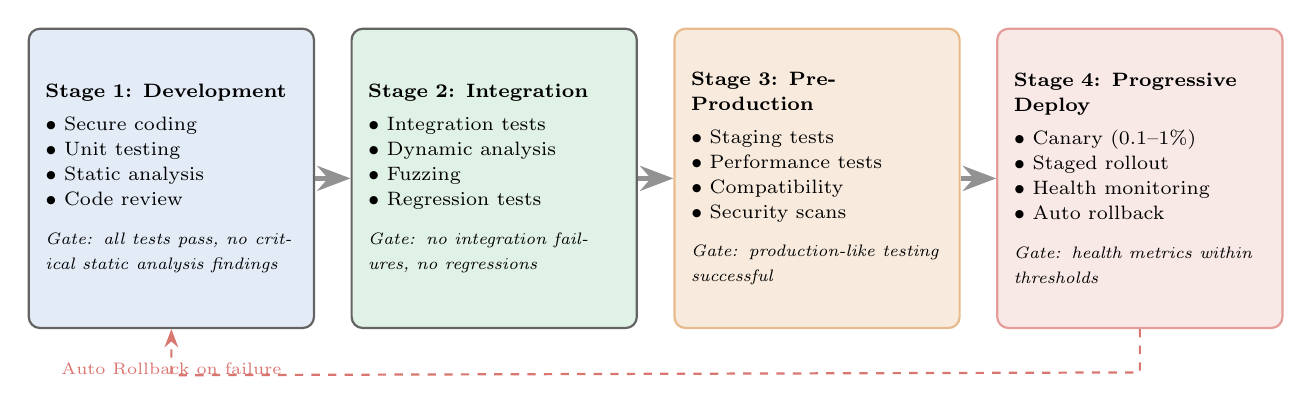
\begin{tikzpicture}[
  font=\fontsize{7pt}{9pt}\selectfont,
  >=Stealth,
  sbox/.style={
    rectangle, rounded corners=4pt, draw=cgray, thick,
    minimum width=3.4cm, minimum height=3.8cm,
    text width=3.2cm, align=left, inner sep=6pt
  },
  arr/.style={-{Stealth}, line width=2pt},
  rarr/.style={-{Stealth}, thick, dashed, cred!70}
]

  %% ── Stage x-centres ──────────────────────────────────────────────────────
  \def\xs{0}     %% Stage 1
  \def\xi{4.1}   %% Stage 2
  \def\xp{8.2}   %% Stage 3
  \def\xd{12.3}  %% Stage 4

  %% ── Stage boxes ──────────────────────────────────────────────────────────
  \node[sbox, fill=cblue!15] (s1) at (\xs, 0) {
    \textbf{Stage 1: Development}\\[3pt]
    $\bullet$ Secure coding\\
    $\bullet$ Unit testing\\
    $\bullet$ Static analysis\\
    $\bullet$ Code review\\[5pt]
    \textit{\fontsize{6pt}{7.5pt}\selectfont Gate: all tests pass,
    no critical static analysis findings}
  };

  \node[sbox, fill=cgreen!15] (s2) at (\xi, 0) {
    \textbf{Stage 2: Integration}\\[3pt]
    $\bullet$ Integration tests\\
    $\bullet$ Dynamic analysis\\
    $\bullet$ Fuzzing\\
    $\bullet$ Regression tests\\[5pt]
    \textit{\fontsize{6pt}{7.5pt}\selectfont Gate: no integration
    failures, no regressions}
  };

  \node[sbox, fill=corange!15, draw=corange!50] (s3) at (\xp, 0) {
    \textbf{Stage 3: Pre-Production}\\[3pt]
    $\bullet$ Staging tests\\
    $\bullet$ Performance tests\\
    $\bullet$ Compatibility\\
    $\bullet$ Security scans\\[5pt]
    \textit{\fontsize{6pt}{7.5pt}\selectfont Gate: production-like
    testing successful}
  };

  \node[sbox, fill=cred!12, draw=cred!50] (s4) at (\xd, 0) {
    \textbf{Stage 4: Progressive Deploy}\\[3pt]
    $\bullet$ Canary (0.1--1\%)\\
    $\bullet$ Staged rollout\\
    $\bullet$ Health monitoring\\
    $\bullet$ Auto rollback\\[5pt]
    \textit{\fontsize{6pt}{7.5pt}\selectfont Gate: health metrics
    within thresholds}
  };

  %% ── Forward arrows ───────────────────────────────────────────────────────
  \draw[arr, color=cgray!70] (s1.east) -- (s2.west);
  \draw[arr, color=cgray!70] (s2.east) -- (s3.west);
  \draw[arr, color=cgray!70] (s3.east) -- (s4.west);

  %% ── Auto-rollback arc (runs below the boxes) ─────────────────────────────
  \draw[rarr]
    (s4.south) -- ++(0,-0.55)
    -- (\xs, {-2.5})
    -- (s1.south)
    node[midway, below, font=\fontsize{6pt}{7.5pt}\selectfont,
         text=cred!70]{Auto Rollback on failure};

\end{tikzpicture}
\caption{Four-stage software assurance framework for update delivery. Each stage
  includes validation activities and formal quality gates. Automated monitoring
  during progressive deployment triggers rollback if health metrics indicate issues.}
\label{fig:framework}
\end{figure*}

\subsection{Stage Details}

\textbf{Stage 1 (Development)}: Secure coding, comprehensive unit tests, automated static
analysis, and peer code review. \textit{Quality Gate}: all tests pass, no critical static
analysis findings.

\textbf{Stage 2 (Integration)}: Integration testing, dynamic analysis with instrumentation,
automated fuzzing with malformed inputs, and comprehensive regression testing.
\textit{Quality Gate}: no integration failures, no regressions.

\textbf{Stage 3 (Pre-Production)}: Staging environment testing mirroring production,
performance testing under realistic load, compatibility testing across supported platforms.
\textit{Quality Gate}: production-like testing successful.

\textbf{Stage 4 (Progressive Deployment)}: Canary deployment (0.1--1\%), intensive health
monitoring, progressive expansion (5\%, 10\%, 25\%, 50\%, 100\%), automated pause and
rollback on threshold violations.
\textit{Quality Gate}: health metrics within acceptable thresholds at each stage.

\subsection{Automated Monitoring and Response}

Key health metrics to monitor: system crash and reboot rates; application error rates;
performance metrics (response time, throughput); and security alert rates. Machine
learning-based anomaly detection should identify significant post-update deviations from
baseline behavior~\cite{basiri2021teaching}. Automated response thresholds: minor anomalies
trigger investigation alerts; moderate issues pause further deployment; severe issues
trigger immediate automated rollback.

\subsection{Risk-Based Tailoring}

Kernel-mode drivers, security-critical components, and critical infrastructure updates
(high-risk) undergo the most rigorous validation with extended staging periods and
heightened monitoring. Application-level updates (medium-risk) may proceed through stages
more rapidly if testing shows no issues. Minor updates (documentation, cosmetic UI) may use
abbreviated validation.

\section{Discussion}

\subsection{The Automation Paradox}

The CrowdStrike incident exemplifies a fundamental paradox: automation simultaneously
enables unprecedented capabilities and amplifies failure consequences. Automated deployment
requires automated validation, monitoring, and recovery---the sophistication of the quality
assurance mechanisms must match the sophistication of the deployment
mechanism~\cite{basiri2021teaching}.

\subsection{Software as Critical Infrastructure}

The incident's impact across aviation, healthcare, and financial services demonstrates that
software has become critical infrastructure~\cite{householder2020cvd}. This raises
questions about regulatory oversight for software affecting critical infrastructure,
vendor liability for defective software causing widespread damage, and mandatory incident
disclosure requirements.

\subsection{The Human Element}

While this paper emphasizes technical controls, the human element remains central. The
incident likely resulted from human decisions: developers writing defective code, reviewers
missing errors, managers prioritizing schedule over quality~\cite{rajapakse2022challenges}.
Effective software assurance requires investing in training and skills, maintaining
sustainable pace, fostering psychological safety, and building diverse teams that bring
different perspectives to quality review.

\begin{table*}[t]
\caption{Comparison of Assurance Approaches: Traditional vs.\ Proposed Framework.}
\label{tab:comparison}
\small
\setlength{\tabcolsep}{5pt}
\begin{tabularx}{\textwidth}{@{}p{3.0cm}XX@{}}
\toprule
\textbf{Aspect} & \textbf{Traditional Approach} & \textbf{Proposed Framework} \\
\midrule
Testing Scope       & Development phase only           & Continuous through deployment \\
Deployment Strategy & Full simultaneous rollout         & Progressive staged deployment \\
Monitoring          & Manual after-deployment checks   & Automated real-time anomaly detection \\
Rollback            & Manual, takes hours/days         & Automated, completes in minutes \\
Quality Gates       & Single pre-release gate          & Multi-stage gates throughout pipeline \\
Risk Assessment     & One-time pre-deployment          & Continuous throughout lifecycle \\
Recovery Capability & Reactive manual remediation      & Proactive automated recovery \\
Metrics             & Code coverage, bug counts        & Health metrics, deployment success rates \\
\bottomrule
\end{tabularx}
\end{table*}

\section{Conclusion}

The July 2024 CrowdStrike Falcon Sensor update failure provides sobering lessons about
software assurance in the modern era. Our analysis reveals contributing technical failures
(defective kernel driver code that static analysis, code review, dynamic testing, and
fuzzing should have detected), process failures (absent staged rollout and automated
monitoring), and organizational factors (deployment pressure and complacency about update
risks).

Six key takeaways emerge: (1)~Software assurance must extend throughout the entire
lifecycle with particular emphasis on update delivery; (2)~Automated deployment requires
automated validation, monitoring, and recovery; (3)~Staged rollout with per-phase
monitoring enables early issue detection; (4)~Even reputable vendors can release defective
updates---validation is essential; (5)~Technical controls alone are insufficient without
organizational culture and training; and (6)~Software failures affect human welfare,
making assurance a moral imperative.

The convergence of this incident with NIST SP 800-53 revisions emphasizing software update
controls suggests the security community recognizes these gaps. Software assurance is not a
checkbox, not a phase to rush through. It is the discipline ensuring that when people trust
their health, safety, and livelihoods to software systems, that trust is well-founded.

\sloppy
\bibliographystyle{ACM-Reference-Format}
\begin{thebibliography}{19}
\bibitem{plummer2024crowdstrike} R.~Plummer and T.~Gerken. 2024. CrowdStrike and Microsoft: What we know about global IT outage. \textit{BBC News}.
\bibitem{siddiqui2024crowdstrike} Z.~Siddiqui. 2024. CrowdStrike update that caused global outage likely skipped checks. \textit{Reuters}.
\bibitem{nist2024sp80053} NIST. 2024. NIST revises security and privacy control catalog. \textit{NIST News} (August 2024).
\bibitem{yankel2022devsecops} J.~Yankel and H.~Yasar. 2022. 5 Challenges to Implementing DevSecOps. \textit{SEI Blog}, Carnegie Mellon University.
\bibitem{crowdstrike2024incident} CrowdStrike. 2024. Falcon Content Update Remediation and Guidance Hub. \textit{CrowdStrike Support}.
\bibitem{microsoft2024crowdstrike} D.~Weston. 2024. Helping our customers through the CrowdStrike outage. \textit{Microsoft Blog}.
\bibitem{shahin2021continuous} M.~Shahin, M.~A.~Babar, and L.~Zhu. 2021. \textit{J.\ Systems and Software} 169, 110683.
\bibitem{rajapakse2022challenges} R.~N.~Rajapakse et al. 2022. \textit{Empirical Software Engineering} 27, 3, 1--41.
\bibitem{xu2021empirical} B.~Xu et al. 2021. \textit{Empirical Software Engineering} 26, 4, 1--43.
\bibitem{householder2020cvd} A.~D.~Householder et al. 2021. \textit{CERT Guide to Coordinated Vulnerability Disclosure}. CMU/SEI-2021-SR-001.
\bibitem{ladisa2023sok} P.~Liguori et al. 2023. SoK: Analysis of Software Supply Chain Security. \textit{ACM ASIA CCS '23}, 485--499.
\bibitem{ohm2020backstabbers} M.~Ohm et al. 2020. Backstabber's Knife Collection. \textit{DIMVA 2020}, 23--43.
\bibitem{basiri2021teaching} A.~Basiri et al. 2021. Teaching Chaos Engineering. \textit{IEEE Software} 38, 1, 4--9.
\bibitem{graham2021cloudflare} J.~Graham-Cumming. 2021. Cloudflare outage analysis. \textit{Cloudflare Blog}.
\bibitem{janardhan2021bgp} S.~Janardhan. 2021. More details about the October 4 outage. \textit{Facebook Engineering Blog}.
\bibitem{frei2021analysis} S.~Frei et al. 2021. 0-Day Patch: Exposure Delay Analysis. \textit{Technical Report}, armasuisse.
\bibitem{forsgren2021accelerate} N.~Forsgren et al. 2021. \textit{2021 State of DevOps Report}. Puppet and CircleCI.
\bibitem{smith2021investigating} B.~Smith and L.~Williams. 2021. \textit{Information and Software Technology} 138, 106618.
\bibitem{madou2024coding} M.~Madou. 2024. Poor coding patterns can lead to big security problems. \textit{Secure Code Warrior}.
\end{thebibliography}

\end{document}
